\documentclass[man,12pt,floatsintext,donotrepeattitle]{apa7}

\usepackage{latexml}  % \iflatexml: true under LaTeXML/oxide, false under pdflatex
\usepackage[american]{babel}
\usepackage{csquotes}
\usepackage{amsmath,amssymb}
\usepackage{amsthm}
\usepackage{booktabs}
\usepackage{graphicx}
\usepackage{xcolor}
\usepackage{subcaption}
\usepackage[most]{tcolorbox}
\usetikzlibrary{positioning, arrows.meta, fit, calc, decorations.pathreplacing}
\usepackage{needspace}
\usepackage[style=apa,backend=biber]{biblatex}
\usepackage{xr}
\externaldocument{draft6}
\externaldocument{supplement1}
\addbibresource{refs.bib}
\usepackage{nameref}
\hypersetup{
  hidelinks,
  pdftitle={Supplement 4: Exploratory Domain Analysis and a Withdrawn Statistic},
  pdfauthor={Joseph Corneli},
  pdfsubject={Permutation-propagators in cellular automata},
  pdfkeywords={cellular automata, rule evolution, Langton's lambda,
    self-modifying systems, edge of chaos, artificial life, permutation
    operators, exhaustive classification, domain walls}
}

\newcommand{\sig}{\sigma}
\newcommand{\bit}[1]{\mathrm{bit}[#1]}
% Sections are unnumbered in apa7 `man' mode, so \ref{sec:..} is empty;
% cross-reference sections by name instead.
\newcommand{\secref}[1]{\emph{\nameref{#1}}}
\newtheorem{theorem}{Theorem}
\newtheorem{corollary}{Corollary}
\newtheorem{proposition}{Proposition}
% Named distinctly: `definition' is a tcolorbox environment in the main
% paper, and this file is \input into packet.tex under docmute.
\newtheorem{scoredef}{Definition}
% Typed boxes are tcolorboxes (TikZ drawings); a converter would render them
% as fixed-geometry SVG rather than text. Define semantic equivalents instead.
% NB: \newif must sit outside the guard -- TeX counts \if tokens when skipping.
\newif\ifpaperboxfold
\iflatexml
  % html-boxes.tex -- converter-side definitions of the paper's typed boxes.
%
% WHY: the print versions of these boxes are tcolorboxes, which are drawn with
% TikZ. latexml-oxide converts TikZ faithfully -- by rendering it as SVG. That
% turns 94% of Supplement 1 and 72% of Supplement 2 into fixed-geometry
% pictures: they do not reflow, they do not scale to a narrow screen, and the
% text inside them is not HTML.
%
% So under a converter we skip tcolorbox entirely and define the same
% environments as ordinary theorem-like blocks. LaTeXML and oxide both emit
% these as <div class="ltx_theorem ltx_theorem_NAME"> with a real title, a real
% counter and a real anchor -- semantic HTML that reflows and can be styled.
%
% Input this from inside an \iflatexml branch, then declare the boxes the
% document actually uses:
%
%     \iflatexml
%       % html-boxes.tex -- converter-side definitions of the paper's typed boxes.
%
% WHY: the print versions of these boxes are tcolorboxes, which are drawn with
% TikZ. latexml-oxide converts TikZ faithfully -- by rendering it as SVG. That
% turns 94% of Supplement 1 and 72% of Supplement 2 into fixed-geometry
% pictures: they do not reflow, they do not scale to a narrow screen, and the
% text inside them is not HTML.
%
% So under a converter we skip tcolorbox entirely and define the same
% environments as ordinary theorem-like blocks. LaTeXML and oxide both emit
% these as <div class="ltx_theorem ltx_theorem_NAME"> with a real title, a real
% counter and a real anchor -- semantic HTML that reflows and can be styled.
%
% Input this from inside an \iflatexml branch, then declare the boxes the
% document actually uses:
%
%     \iflatexml
%       % html-boxes.tex -- converter-side definitions of the paper's typed boxes.
%
% WHY: the print versions of these boxes are tcolorboxes, which are drawn with
% TikZ. latexml-oxide converts TikZ faithfully -- by rendering it as SVG. That
% turns 94% of Supplement 1 and 72% of Supplement 2 into fixed-geometry
% pictures: they do not reflow, they do not scale to a narrow screen, and the
% text inside them is not HTML.
%
% So under a converter we skip tcolorbox entirely and define the same
% environments as ordinary theorem-like blocks. LaTeXML and oxide both emit
% these as <div class="ltx_theorem ltx_theorem_NAME"> with a real title, a real
% counter and a real anchor -- semantic HTML that reflows and can be styled.
%
% Input this from inside an \iflatexml branch, then declare the boxes the
% document actually uses:
%
%     \iflatexml
%       \input{html-boxes}
%       \NewHTMLBox{definition}{Definition}{1}   % 1 = takes a {title} argument
%       \NewHTMLBox{theorem}{Theorem}{0}         % 0 = no title argument
%     \else
%       ... the tcolorbox definitions ...
%     \fi
%
% The [label={...}] option each box carries in the sources is honoured, so
% \ref and \autoref into the boxes keep working.

\usepackage{amsthm}
\usepackage{keyval}

% This file is \input, not a package, so `@` is not a letter here: everything
% touching \define@key or \@empty must sit inside \makeatletter.
\makeatletter

% Option keys. Only `label` does anything; the rest are print-layout keys that
% appear in the sources (fold, breakable=false) and must be absorbed silently.
\define@key{htmlbox}{label}{\def\htmlboxlabel{#1}}
\define@key{htmlbox}{fold}[]{}
\define@key{htmlbox}{unfold}[]{}
\define@key{htmlbox}{breakable}[]{}

\newcommand{\htmlboxsetup}[1]{%
  \def\htmlboxlabel{}%
  \def\htmlbox@opts{#1}%
  \ifx\htmlbox@opts\@empty\else\setkeys{htmlbox}{#1}\fi
  \ifx\htmlboxlabel\@empty\else\expandafter\label\expandafter{\htmlboxlabel}\fi}
\makeatother

% \NewHTMLBox{envname}{Heading}{1 if it takes a mandatory {title}, else 0}
\newcommand{\NewHTMLBox}[3]{%
  % amsthm's default `plain' style italicises the body, which is wrong for
  % findings and worked examples that are pages of prose. `definition' style
  % keeps the body upright and only bolds the heading.
  \theoremstyle{definition}%
  \newtheorem{htmlbox#1}{#2}%
  \ifnum#3=1\relax
    \NewDocumentEnvironment{#1}{O{} m}%
      {\begin{htmlbox#1}[##2]\htmlboxsetup{##1}}%
      {\end{htmlbox#1}}%
  \else
    \NewDocumentEnvironment{#1}{O{}}%
      {\begin{htmlbox#1}\htmlboxsetup{##1}}%
      {\end{htmlbox#1}}%
  \fi}

% Present in the print branch; harmless no-ops here so stray uses do not break.
\providecommand{\foldmark}{}
\providecommand{\thetcbcounter}{}
\makeatletter
\@ifundefined{ifpaperboxfold}{\newif\ifpaperboxfold}{}
\makeatother
\endinput

%       \NewHTMLBox{definition}{Definition}{1}   % 1 = takes a {title} argument
%       \NewHTMLBox{theorem}{Theorem}{0}         % 0 = no title argument
%     \else
%       ... the tcolorbox definitions ...
%     \fi
%
% The [label={...}] option each box carries in the sources is honoured, so
% \ref and \autoref into the boxes keep working.

\usepackage{amsthm}
\usepackage{keyval}

% This file is \input, not a package, so `@` is not a letter here: everything
% touching \define@key or \@empty must sit inside \makeatletter.
\makeatletter

% Option keys. Only `label` does anything; the rest are print-layout keys that
% appear in the sources (fold, breakable=false) and must be absorbed silently.
\define@key{htmlbox}{label}{\def\htmlboxlabel{#1}}
\define@key{htmlbox}{fold}[]{}
\define@key{htmlbox}{unfold}[]{}
\define@key{htmlbox}{breakable}[]{}

\newcommand{\htmlboxsetup}[1]{%
  \def\htmlboxlabel{}%
  \def\htmlbox@opts{#1}%
  \ifx\htmlbox@opts\@empty\else\setkeys{htmlbox}{#1}\fi
  \ifx\htmlboxlabel\@empty\else\expandafter\label\expandafter{\htmlboxlabel}\fi}
\makeatother

% \NewHTMLBox{envname}{Heading}{1 if it takes a mandatory {title}, else 0}
\newcommand{\NewHTMLBox}[3]{%
  % amsthm's default `plain' style italicises the body, which is wrong for
  % findings and worked examples that are pages of prose. `definition' style
  % keeps the body upright and only bolds the heading.
  \theoremstyle{definition}%
  \newtheorem{htmlbox#1}{#2}%
  \ifnum#3=1\relax
    \NewDocumentEnvironment{#1}{O{} m}%
      {\begin{htmlbox#1}[##2]\htmlboxsetup{##1}}%
      {\end{htmlbox#1}}%
  \else
    \NewDocumentEnvironment{#1}{O{}}%
      {\begin{htmlbox#1}\htmlboxsetup{##1}}%
      {\end{htmlbox#1}}%
  \fi}

% Present in the print branch; harmless no-ops here so stray uses do not break.
\providecommand{\foldmark}{}
\providecommand{\thetcbcounter}{}
\makeatletter
\@ifundefined{ifpaperboxfold}{\newif\ifpaperboxfold}{}
\makeatother
\endinput

%       \NewHTMLBox{definition}{Definition}{1}   % 1 = takes a {title} argument
%       \NewHTMLBox{theorem}{Theorem}{0}         % 0 = no title argument
%     \else
%       ... the tcolorbox definitions ...
%     \fi
%
% The [label={...}] option each box carries in the sources is honoured, so
% \ref and \autoref into the boxes keep working.

\usepackage{amsthm}
\usepackage{keyval}

% This file is \input, not a package, so `@` is not a letter here: everything
% touching \define@key or \@empty must sit inside \makeatletter.
\makeatletter

% Option keys. Only `label` does anything; the rest are print-layout keys that
% appear in the sources (fold, breakable=false) and must be absorbed silently.
\define@key{htmlbox}{label}{\def\htmlboxlabel{#1}}
\define@key{htmlbox}{fold}[]{}
\define@key{htmlbox}{unfold}[]{}
\define@key{htmlbox}{breakable}[]{}

\newcommand{\htmlboxsetup}[1]{%
  \def\htmlboxlabel{}%
  \def\htmlbox@opts{#1}%
  \ifx\htmlbox@opts\@empty\else\setkeys{htmlbox}{#1}\fi
  \ifx\htmlboxlabel\@empty\else\expandafter\label\expandafter{\htmlboxlabel}\fi}
\makeatother

% \NewHTMLBox{envname}{Heading}{1 if it takes a mandatory {title}, else 0}
\newcommand{\NewHTMLBox}[3]{%
  % amsthm's default `plain' style italicises the body, which is wrong for
  % findings and worked examples that are pages of prose. `definition' style
  % keeps the body upright and only bolds the heading.
  \theoremstyle{definition}%
  \newtheorem{htmlbox#1}{#2}%
  \ifnum#3=1\relax
    \NewDocumentEnvironment{#1}{O{} m}%
      {\begin{htmlbox#1}[##2]\htmlboxsetup{##1}}%
      {\end{htmlbox#1}}%
  \else
    \NewDocumentEnvironment{#1}{O{}}%
      {\begin{htmlbox#1}\htmlboxsetup{##1}}%
      {\end{htmlbox#1}}%
  \fi}

% Present in the print branch; harmless no-ops here so stray uses do not break.
\providecommand{\foldmark}{}
\providecommand{\thetcbcounter}{}
\makeatletter
\@ifundefined{ifpaperboxfold}{\newif\ifpaperboxfold}{}
\makeatother
\endinput

  \NewHTMLBox{workedexample}{Worked example}{1}
  \NewHTMLBox{empiricalfinding}{Empirical finding}{1}
  \NewHTMLBox{observation}{Observation}{1}
\else
\newtcolorbox[auto counter]{workedexample}[2][]{%
  enhanced,
  breakable,
  colback=green!6,
  colframe=green!45!black,
  boxrule=0.7pt,
  arc=1.5mm,
  left=2.5mm,
  right=2.5mm,
  top=1.5mm,
  bottom=1.5mm,
  fonttitle=\bfseries,
  title={Worked example~\thetcbcounter: #2},
  #1}

% --- typed boxes for compression -------------------------------------------
% Auto-box existing amsthm theorems/definitions (no source change; keeps refs).
\tcolorboxenvironment{theorem}{%
  enhanced, breakable, colback=blue!5, colframe=blue!55!black,
  boxrule=0.7pt, arc=1.5mm, left=2.5mm, right=2.5mm, top=1.5mm, bottom=1.5mm}
\tcolorboxenvironment{definition}{%
  enhanced, breakable, colback=violet!6, colframe=violet!55!black,
  boxrule=0.7pt, arc=1.5mm, left=2.5mm, right=2.5mm, top=1.5mm, bottom=1.5mm}
% Corollaries auto-boxed like theorems (blue). Empirical findings are amber:
% observed (not proved) claims live here, the validated home for rewritten results.
\tcolorboxenvironment{corollary}{%
  enhanced, breakable, colback=blue!5, colframe=blue!55!black,
  boxrule=0.7pt, arc=1.5mm, left=2.5mm, right=2.5mm, top=1.5mm, bottom=1.5mm}
\tcolorboxenvironment{proposition}{%
  enhanced, breakable, colback=blue!5, colframe=blue!55!black,
  boxrule=0.7pt, arc=1.5mm, left=2.5mm, right=2.5mm, top=1.5mm, bottom=1.5mm}
\newtcolorbox[auto counter]{empiricalfinding}[2][]{%
  enhanced, breakable, colback=orange!7, colframe=orange!65!black,
  boxrule=0.7pt, arc=1.5mm, left=2.5mm, right=2.5mm, top=1.5mm, bottom=1.5mm,
  fonttitle=\bfseries, title={Empirical finding~\thetcbcounter: #2}, #1}
% Observations (teal): consequences/remarks pulled out of definitions and prose.
\newtcolorbox[auto counter]{observation}[2][]{%
  enhanced, breakable, colback=teal!7, colframe=teal!55!black,
  boxrule=0.7pt, arc=1.5mm, left=2.5mm, right=2.5mm, top=1.5mm, bottom=1.5mm,
  fonttitle=\bfseries, title={Observation~\thetcbcounter: #2}, #1}
\fi

\title{Supplement 4: Exploratory Domain Analysis and a Withdrawn Statistic}
\shorttitle{Rule-Rewriting Cellular Automata}
\authorsnames{Joseph Corneli}
\authorsaffiliations{{Oxford Brookes University, Oxford OX3 0BP, United Kingdom},
  {Hyperreal Enterprises Ltd, United Kingdom}}
\note{Corresponding author: Joseph Corneli,
  \href{mailto:jcorneli@brookes.ac.uk}{jcorneli@brookes.ac.uk}.}

\abstract{%
We study a two-layer cellular automaton in which each cell carries both a
phenotype state and an eight-bit rule. A permutation $\sig$ of the eight
displayed truth-table positions defines an operator $P_\sig$ on those rules by
$\bit{\sig(p)} := \lnot\,\bit{p}$. The resulting family contains
$8! = 40{,}320$ permutation-propagators and is exhaustively classifiable.

The exact, machine-checked classification is that $P_\sig$ has a fixed rule
exactly when every cycle of $\sig$ is even; an all-even permutation with $k$
cycles has $2^k$ fixed rules; and every fixed rule is balanced, with Langton
activity $\lambda=1/2$. In a census of the spatially coupled dynamics, every
odd-cycle operator is genotype-alive under the stated finite-run protocol,
whereas every all-even cycle type contains both sustaining and collapsing
operators.

Within the wrap-rotation subfamily, coprime rotations sustain high diversity
while the other nontrivial rotations collapse in the runs tested. A finite-size
scan finds a broad, drifting crossover rather than evidence of a sharpening
critical point. Filamentary boundaries show elevated genotype rewriting and,
in one sampled coexisting-domain field, separate genotypically distinct rule
populations at matched activity. A
directed-transport statistic on those boundaries does not survive its own
controls---mask and measure are derived from the same thresholded field---and is
withdrawn here, together with the analysis that rested on it. In its place a
causal measure, perturbing one cell and tracking the divergence against a
matched control that differs only in the phenotype-to-genotype edge, shows that
this feedback roughly doubles how far a perturbation travels, and places the
construction between elementary rules $90$ and $54$ on a damage-spreading scale
calibrated against rules of known regime. Temporal braids and a phenotype-reading
construction provide two reproducible ways to sustain structure beyond the
bare operator.}
\keywords{cellular automata, rule evolution, Langton's lambda,
self-modifying systems, edge of chaos, artificial life, permutation operators,
exhaustive classification, domain walls}

% Artificial Life asks for the abstract and keywords on the cover page and the
% main text on page 2. In apa7 manuscript mode, suppress the page break that
% normally separates the title page from the abstract; retain the following
% page break before the main text.
% See draft8.tex: print-only title-page patches, guarded for converters.
\iflatexml\else
\makeatletter
\patchcmd{\maketitle}{\vspace*{4\baselineskip}}{\vspace*{\baselineskip}}%
  {}{\PackageError{draft5}{Could not compact title-page spacing}{}}
\patchcmd{\maketitle}{\newpage}{\vspace{0pt}}%
  {}{\PackageError{draft5}{Could not place abstract on title page}{}}
\makeatother
\fi

% Float numbers carry the supplement number so they are unambiguous both
% standalone and when bound into packet.tex.
\renewcommand{\thefigure}{S4.\arabic{figure}}
\renewcommand{\thetable}{S4.\arabic{table}}

\begin{document}
\maketitle

This second supplement carries three strands of the companion paper that are reported
in full here rather than in the main text: the spatial domain structure of the
genotype field and its filamentary boundaries; a measure of information
transport along those boundaries that we built, validated against three nulls,
and then withdrew; and the domain/particle reading that motivated both.

The main paper's claim is about a single edge of chaos, reached by causal
measurement rather than by tuning a parameter. The material here is not that. It
is a real spatial structure that we spent some time mistaking for a third edge,
and the record of how that mistake was made and caught. We report it at length
because the failed construction is a natural one to reach for, and because the
geometry-preserving nulls that appear to guard against its failure do not.

Figure, section and empirical-finding numbers below that are not preceded by
``Supplement'' refer to the main paper, and resolve to its numbering.

\section{Domain Structure and Filamentary Boundaries}
\label{supp:domains}

The finite-size scan of the main paper (\emph{Supplement 1, Box~\ref{find:crossover}},
Figure~\ref{fig:phase}) finds a broad crossover rather than a critical point. We then asked whether the
sustained diversity is spatially organised. It is.

\begin{empiricalfinding}[label={find:littoral}]{A finite-width intermediate-activity band}
An intermediate-activity band ($0.15 \le a_G \le 0.60$) has a \emph{lower} edge
robustly at $q \approx 0.1$---stable under both system size and threshold---while
its upper edge is threshold-dependent, because $a_G$ saturates gradually rather
than jumping (the band spans $q \approx 0.1$ to $0.4$--$0.5$). This finite-width
crossover is what we call a \emph{littoral edge}: a descriptive name for a shore
of finite width, not a thermodynamic phase boundary.
\end{empiricalfinding}

\begin{scoredef}[Isolated-rule activity score]\label{def:activity}
The \emph{activity score} of a rule is the mean per-step cell-change fraction
over the final $150$ steps of a $300$-step ordinary ECA run on a periodic line
of width $300$. Every rule uses the same density-$1/2$ pseudorandom initial
condition (seed $1$). This finite-run measure is distinct from the static
truth-table balance $\lambda$ (\secref{sec:lambda}). Ordered rules score near
$0$; Rule~$110$ scores approximately $0.42$, and several standard chaotic rules
score approximately $0.50$. The score orders activity levels but does not by
itself distinguish complex from chaotic dynamics.
\end{scoredef}

Tinting the genotype by this score (Figure~\ref{fig:tint}) resolves the
intermediate field into coexisting low- and high-activity domains whose
boundaries trace filamentary sets through $1{+}1$-dimensional spacetime---objects
\emph{analogous to} the domain boundaries of computational mechanics
\parencite{crutchfield1989inferring,shalizi2001computational}, here obtained by
thresholding a scalar tint rather than by predictive equivalence.

\begin{empiricalfinding}[label={find:walls}]{Filamentary walls have elevated genotype churn}
The activity field resolves into ordered and chaotic domains separated by
\emph{fractal-like walls} (Figure~\ref{fig:interface}; box-counting dimension
$D \approx 1.5$--$1.7$ over $L = 128$--$768$, a handful of seeds). Those walls are
the locus of elevated \emph{genotypic} change: measuring the row-to-row rewrite
rate by region (Table~\ref{tab:churn}), the wall churn exceeds the chaotic
interior in all $32$ committed operator/width/seed fields and exceeds
\emph{both} interiors in $24$. At $L = 256$, offset $+1$ gives $0.80$ at the
wall against $0.81$ (ordered) and $0.73$ (chaotic); the corresponding wall is
the maximum region for $\sigma=16250374$ and the river. The chaotic domain has
the lowest aggregate churn for every operator and width (and in $29$ of the
$32$ individual fields), so the wall---where ordered abuts chaotic---is
consistently more rewritten than the chaotic interior, though not universally
more than the ordered one. The walls are not compositionally special (no rule
class enriched; Rule~110 is, if anything, depleted), so the distinction is
dynamical rather than a difference in rule composition. The interface analysis
is exploratory: it uses a handful of seeds and a fixed-boundary variant, and
the denser river boundary ($D\approx1.8$ versus $1.5$--$1.7$) is an unmatched
comparison that does not establish an effect of genotype--phenotype coupling.
Whether rewriting transports information \emph{along} the walls is taken up in
\secref{sec:eoc-compute}; the answer there is negative.
\end{empiricalfinding}

The partition is by activity, so the two sides differ in activity by
construction. The question that is not self-answering is whether they differ in
anything else.

\begin{empiricalfinding}[label={find:matched}]{The domains hold different rules at matched activity}
Restricting to cells whose \emph{individual} activity score lies in a narrow
band, and comparing the distribution over rule identities on the two sides, the
total-variation distance exceeds a noise floor---obtained by randomly halving
the larger group---by $13$ to $25\times$ across bands: $0.489$ against $0.023$
for scores near zero, $0.147$ against $0.011$ in $[0.20,0.35)$, $0.295$ against
$0.020$ in $[0.45,0.55)$, and $0.522$ against $0.021$ above $0.55$. Rule
diversity differs as well: at matched activity in $[0.45,0.55)$ the active
domain holds $24$ distinct rules per thousand cells against the quiet domain's
$38$. Two cells of equal activity belong to systematically different rule
populations according to which domain they occupy, so the partition captures
genotypic structure the activity score does not determine. Measured on the
$q = 0.25$ coexisting-domain field of Figure~\ref{fig:phase}.
\end{empiricalfinding}


\begin{figure}[tb]
\centering
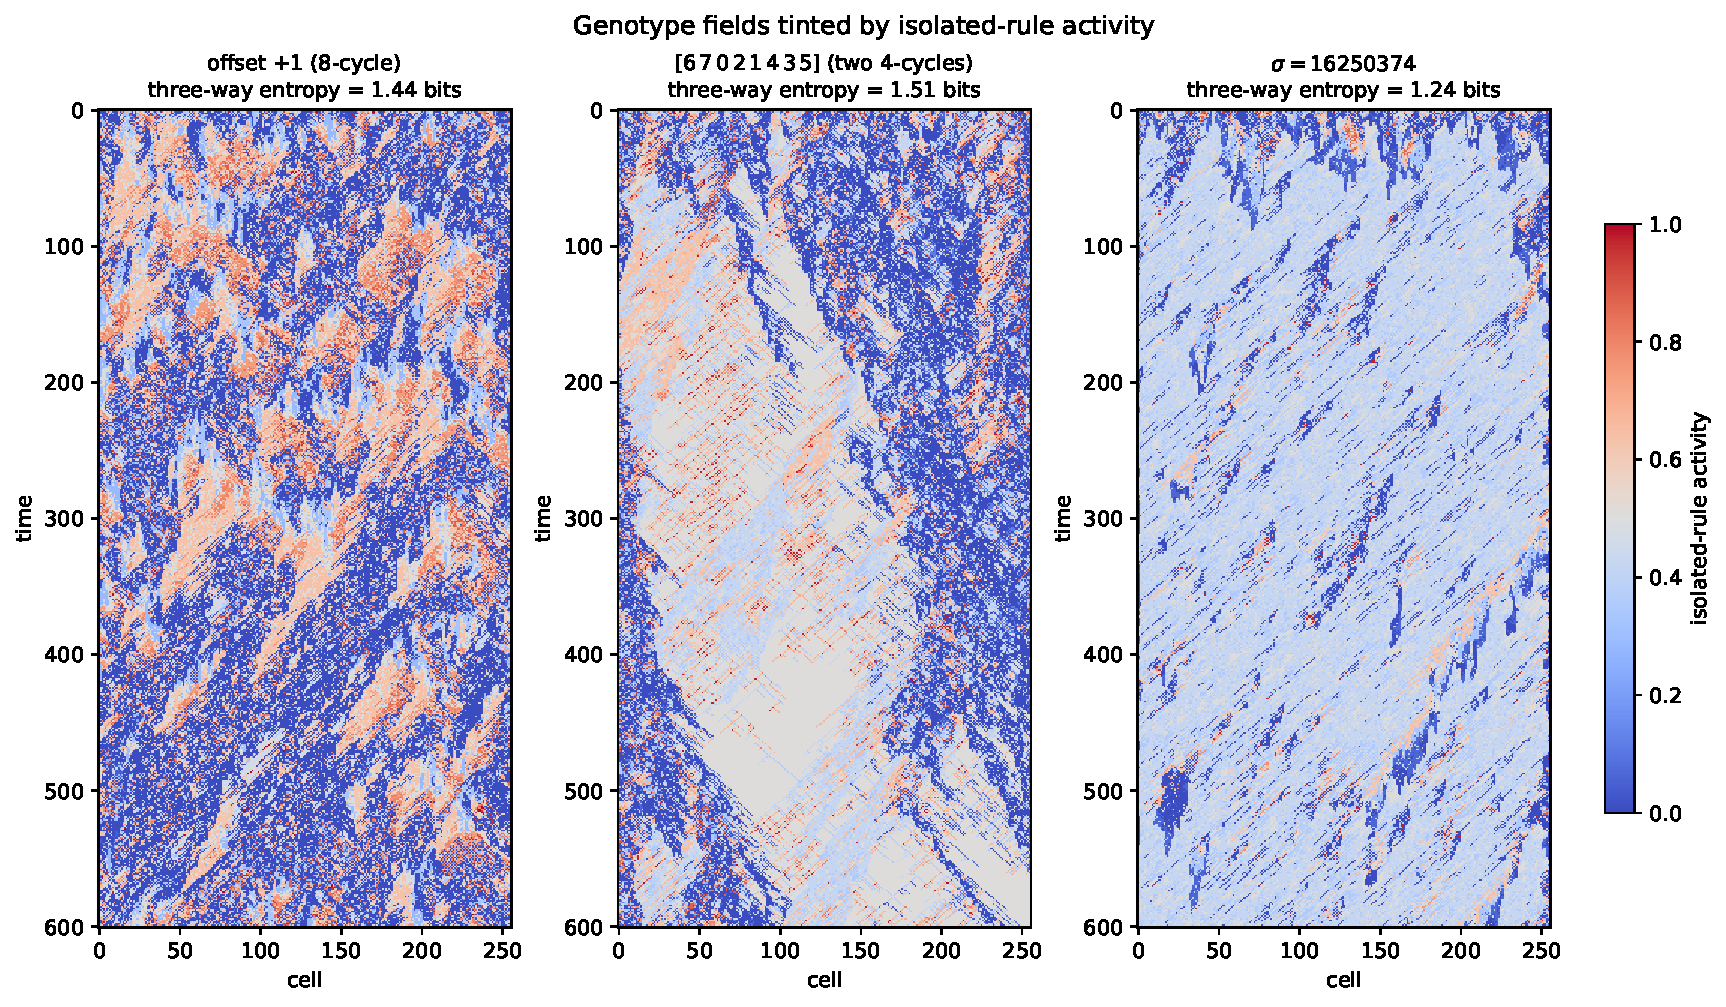
\includegraphics[width=\linewidth]{figures/eoc_tint.pdf}
\caption{\textbf{The genotype as a map of activity regimes.} Genotype spacetime
fields (fixed-boundary variant) tinted by each rule's \emph{isolated-rule
activity score} (Definition~\ref{def:activity}; blue $=$ low near $0$, pale $=$
intermediate near $0.4$, red $=$ high near $0.5$ and above). Which active regime
pairs with the low-activity background depends on the operator, and the three-way
balance differs sharply (entropy in bits, in title): offset $+1$ (the 8-cycle
survivor) mixes low with high-activity chaotic rules in a \emph{fine} texture;
the two-4-cycle $[6\,7\,0\,2\,1\,4\,3\,5]$---the standard-order form of the
historical offset$+2$ exemplar---forms \emph{large coherent}
intermediate-activity domains
with sharp walls, the most balanced regime mix (entropy $1.51$); and
$\sigma = 16250374$ is dominated by the intermediate complex Rule~110. The score
orders the regimes but does not by itself separate complex from chaotic.}
\label{fig:tint}
\end{figure}

\begin{figure}[tb]
\centering
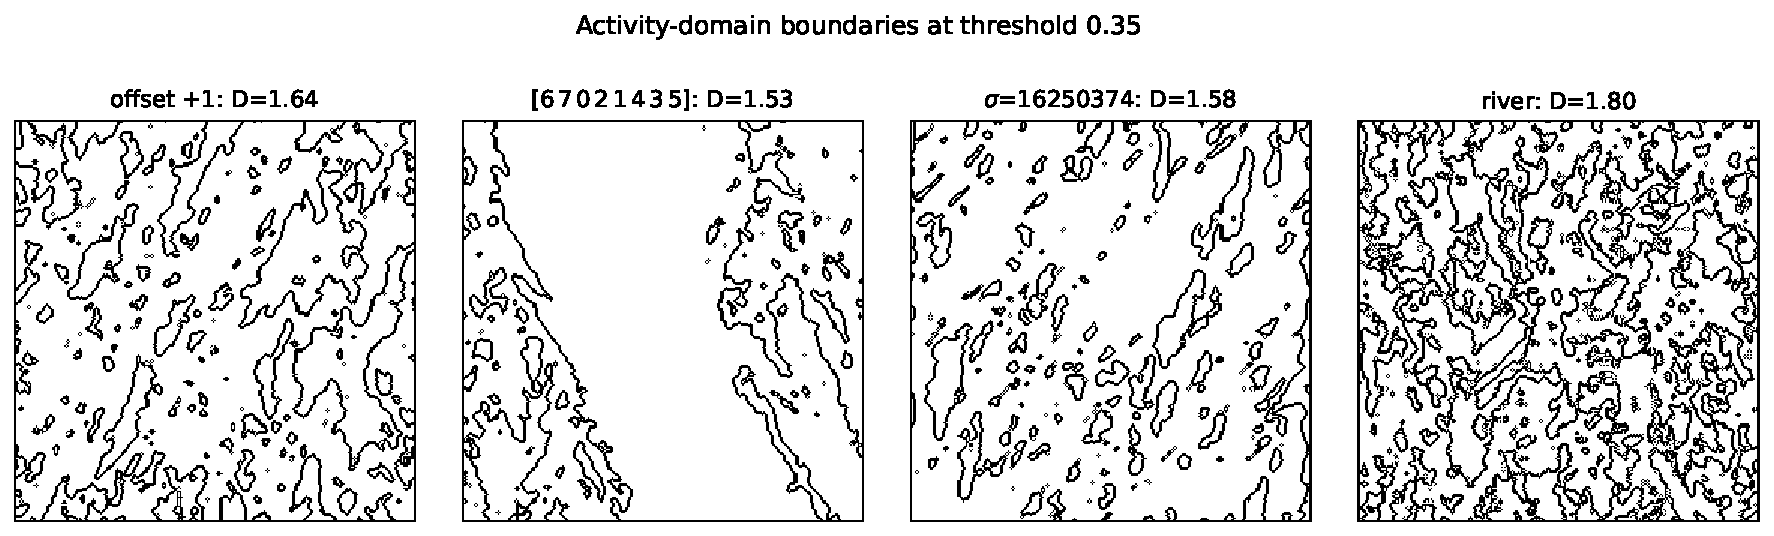
\includegraphics[width=\linewidth]{figures/eoc_interface.pdf}
\caption{\textbf{Activity-domain walls.} The boundary (black) between low- and
high-activity regions, traced through the $1{+}1$-dimensional spacetime diagram at
$L = 256$. Offset $+1$, the two-4-cycle
$[6\,7\,0\,2\,1\,4\,3\,5]$, and $\sigma = 16250374$ carry fractal-like
boundaries ($D \approx 1.5$--$1.6$); the phenotype-coupled river carries a
denser one ($D \approx 1.80$, an unmatched comparison as it couples phenotype).
The dimension is stable across $L = 128$--$768$ (offset $+1\approx1.67$, the
two-4-cycle $\approx1.50$, $\sigma\approx1.54$, and river $\approx1.79$; box
sizes $2$--$64$). Collapsed operators (e.g.\ offset $+4$) carry none. These
walls are also consistently more rewritten than the chaotic-domain interior
(Discussion). Exploratory: a handful of seeds, fixed-boundary variant.}
\label{fig:interface}
\end{figure}

\begin{table}[tb]
\centering
\caption{\textbf{Genotype churn by region}---row-to-row rewrite rate of the rule
field (fraction of cells whose ECA rule changes from the row above), at
$L = 256$, mean over the committed seeds. The wall exceeds the chaotic
interior for every operator; for offset $+1$, the ordered interior is slightly
higher. Wall extraction is the threshold-and-smooth procedure of
Figure~\ref{fig:interface}; reproducible from the generated fields
(\texttt{plot\_eoc\_churn.py}).}
\label{tab:churn}
\begin{tabular}{lccc}
\toprule
Operator & Wall & Ordered interior & Chaotic interior \\
\midrule
offset $+1$          & $0.80$ & $0.81$ & $0.73$ \\
$\sigma = 16250374$  & $0.71$ & $0.68$ & $0.57$ \\
river                & $0.99$ & $0.97$ & $0.96$ \\
\bottomrule
\end{tabular}
\end{table}


\section{A Measure That Failed}
\label{sec:eoc-compute}

If the filaments are domain boundaries they are candidate \emph{wires}. The
natural question is not which rules compose them---in our data the complex rules
are not enriched there---but whether information is \emph{transported along}
them and \emph{combined where they collide} \parencite{mitchell1993revisiting}.
We built an estimator for both, and both are withdrawn. This section reports the
attempt, the controls that appeared to validate it, and the control that
defeated it. We keep it in the main text because the construction is one a
reader might reasonably build, and because the nulls that seem to guard against
its failure do not.

We read both notions off the binary activity field as local transfer entropy
\parencite{lizier2008local}: the apparent transfer entropy from a spatial
neighbour into a cell, conditioned on the cell's own past, scores directed
\emph{transport}; the \emph{synergy} of the two neighbours---their joint
predictive contribution beyond the sum of their separate ones---scores
\emph{combining} (Figure~\ref{fig:eoc-schema}).

A raw on-filament average will not support either claim, and we say why before
using one. The score has two failure modes, and each needs its own null. First,
the plug-in estimator is positively biased, so a field can score positive
transfer entropy with no directed coupling at all; the null for this is a
\emph{source time-shuffle}, which preserves the marginals and the cell's own
past and destroys only the neighbour-to-target coupling. Second---and this is
what defeats the raw statistic---the extracted filament is not a fixed object
across a parameter sweep. It swells from $20\%$ of the field at the bare
operator to $39\%$ under strong noise, at which
point it is no longer a wall, and any on-filament mean drifts toward the field
mean for reasons that have nothing to do with transport. The null for this is a
\emph{mask-matched} draw: the same number of cells, taken anywhere in the
field. We report the difference from that draw and call it \emph{filament-specific}
transport or combining; it is zero when the filament is no better than an
arbitrary set of cells of the same size, and negative when it is worse.

A size-matched draw preserves the filament's extent but not its shape, so we
also ran two nulls that preserve its geometry. The first circularly translates
the mask along $x$ and averages over all displacements beyond the point where a
mask ceases to overlap itself; this retains the mask's exact connectivity,
anisotropy, cell count and per-row occupancy, destroying only its registration
against the field, and it involves no randomness at all. The second scores each
field under the filament extracted from an independent seed at the same sweep
point. Both agree with the size-matched draw to within $0.001$ bits at every
point ($r > 0.999$ across the sweep), and every result below is unchanged under
all three. A filament-shaped region placed generically therefore scores no
differently from scattered cells: what distinguishes the real filament is where
it lies, not the shape of the region measured. We quote the size-matched null
throughout.

The estimator has a third failure mode that no null removes, and it bounds
what follows. Where the activity field is nearly degenerate---almost all cells
in one state---the conditional probabilities driving the score become extreme
and it inflates without bound, and this happens at \emph{either} end. The
genotypically dead offset $+4$ operator is the demonstration. Its genotype
freezes (row-to-row rewrite rate falls to $0$, Empirical
\emph{Supplement 1, Box~\ref{find:braid}}) into a
population that is $98\%$ active, and on that saturated field it records the
largest on-filament transport we measured anywhere: $317\times$ the domain
interior, $+0.59$ bits filament-specific, for an operator that transports
nothing at all. The sparse end behaves the same way, and costs us the most
ordered sample in the sweep below (all blend, $q=0$, $9\%$ active), where the
shuffled surrogate outscores the real field ($+0.144$ against $+0.105$ bits,
$t = -0.71$, $p = 0.49$); that point is bias-dominated and is excluded. Local
transfer entropy is therefore comparable only across fields of similar and
non-degenerate activity density---which is the concrete content of what earlier
drafts recorded as a ``sparsity effect''.

Within these bounds the score behaves as one would hope, and it is worth
recording what that looked like, because it is what made the result credible.
Over the eight seeds of the $q=1$ sweep column, on-filament transfer entropy is
$+0.158 \pm 0.005$ bits against a shuffled surrogate of $+0.002$
($t = 33.5$, $p < 10^{-8}$) and a mask-matched draw of $+0.061$, leaving
$+0.097 \pm 0.005$ bits filament-specific. On the fixed-boundary field of
Figure~\ref{fig:interface} the measure concentrates $5.7\times$ over the domain
interiors; the Rule~$110$-dominated $\sigma = 16250374$ field, taken as a
positive control, shows the same signature ($7.6\times$, filament-specific
$+0.161$ bits). Three nulls agree to within $0.001$ bits, the positive control
behaves as a positive control should, and the effect is large and highly
significant. None of that is evidence, for the reason given next.

\begin{figure}[tb]
\centering
\begin{tikzpicture}
\node[inner sep=0.4pt, draw=black!25] (p) {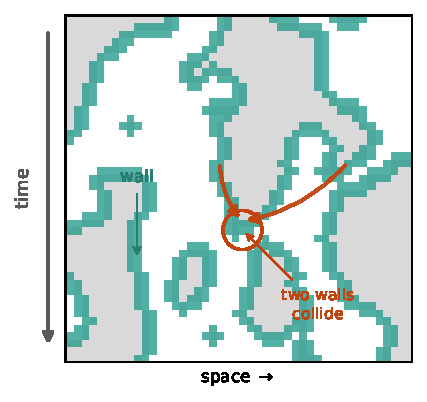
\includegraphics[width=56mm]{figures/eoc_patch.pdf}};
\node[font=\footnotesize, anchor=south] at (p.north)
  {\textbf{(a)} a real patch (offset$+1$): activity domains and their walls};
\end{tikzpicture}
\\[3mm]
\begin{tikzpicture}[font=\footnotesize, >={Stealth[length=1.6mm]},
  cell/.style={draw=black!35, minimum size=7mm, inner sep=0},
  ord/.style={cell, fill=blue!8},
  cha/.style={cell, fill=orange!13},
  wall/.style={cell, fill=teal!20, draw=teal!55!black, thick},
  tgt/.style={cell, fill=teal!45, draw=teal!72!black, very thick},
  te/.style={-{Stealth[length=1.7mm]}, teal!55!black, semithick},
  own/.style={-{Stealth[length=1.7mm]}, black!45, semithick, densely dashed},
  rowlab/.style={font=\scriptsize\itshape, black!55},
  blurb/.style={align=center, font=\footnotesize}]
% Panel (a): transport
\node[blurb] at (0.75,1.75) {\textbf{(b) transport} \\ along a wall};
\node[ord]  (aP0) at (0,0)        {};
\node[wall] (aP1) at (0.75,0)     {};
\node[cha]  (aP2) at (1.5,0)      {};
\node[tgt]  (aC)  at (0.75,-1.05) {$c$};
\node[rowlab] at (-0.62,0)     {$t{-}1$};
\node[rowlab] at (-0.62,-1.05) {$t$};
\draw[own] (aP1) -- (aC);
\draw[te]  (aP0.south) .. controls +(0,-0.5) and +(-0.4,0.2) .. (aC.west);
\node[blurb, text width=36mm, anchor=north] at (0.75,-2.35)
  {\emph{transfer entropy}:\\ a neighbour's past beyond $c$'s own};
% Panel (b): combining
\begin{scope}[xshift=55mm]
\node[blurb] at (0.75,1.75) {\textbf{(c) combining} \\ where walls collide};
\node[wall] (bP0) at (0,0)        {};
\node[ord]  (bP1) at (0.75,0)     {};
\node[wall] (bP2) at (1.5,0)      {};
\node[tgt]  (bC)  at (0.75,-1.05) {$c$};
\draw[decorate, decoration={brace, amplitude=4pt, mirror}, teal!55!black]
  (bP0.north west) -- node[above=2.5pt, font=\scriptsize, teal!55!black] {two walls} (bP2.north east);
\draw[own] (bP1) -- (bC);
\draw[te]  (bP0.south) .. controls +(0,-0.5) and +(-0.4,0.2) .. (bC.west);
\draw[te]  (bP2.south) .. controls +(0,-0.5) and +(0.4,0.2)  .. (bC.east);
\node[blurb, text width=38mm, anchor=north] at (0.75,-2.55)
  {\emph{synergy}:\\ the two walls jointly, beyond their separate effects};
\end{scope}
\end{tikzpicture}
\caption{\textbf{How the two (withdrawn) measures read a filament.} The
estimator illustrated here is the one this section invalidates; the diagram is
retained to make the failure legible. \textbf{(a)}~A real
space--time patch from the synthetic family (offset$+1$): low- and high-activity
domains (white/grey) meet along thin walls (teal), with one wall and one collision
marked. In the schematics each cell $c$ is predicted from its own past (dashed)
and its two spatial neighbours' pasts (teal); tints mark the low- (blue) and
high-activity (orange) domains a wall separates. \textbf{(b)}~\emph{Transport} is
the directed transfer entropy from a neighbour into $c$ beyond $c$'s own past,
which the wall is defined to maximise---the circularity of
\secref{sec:eoc-compute}. \textbf{(c)}~\emph{Combining} is the \emph{synergy} of the
two neighbours---their joint contribution beyond the sum of their separate
ones---probed where two walls collide. History length one; conditioning on the
own past removes what the wall merely carries forward in time.}
\label{fig:eoc-schema}
\end{figure}

\subsection{The measure does not survive its own controls}

The score defined above fails a control we did not originally run. Local
transfer entropy here is computed on the thresholded activity field
$\mathrm{act} = (\mathrm{smooth} > 0.35)$, while the filament mask is the
\emph{gradient of that same field}. The mask therefore marks precisely the cells
at which $\mathrm{act}$ changes, and transfer entropy on a binary field is near
zero except where it changes: $+0.8934$ bits on changed cells against $+0.0080$
elsewhere, the wall capturing changed cells at $163\times$ enrichment. A positive
filament-specific score is guaranteed by the construction rather than by the
dynamics.

Two tests establish this. Holding the mask at $0.35$ and recomputing the measure
at a different threshold collapses the score from $+0.0885$ to $+0.0007$ (at
$0.30$), $-0.0044$ ($0.40$) and $-0.0377$ ($0.50$). Deriving mask and measure
from the same threshold and sweeping it instead recovers the effect at
\emph{every} threshold, growing monotonically from $+0.065$ at $0.25$ to
$+0.173$ at $0.50$. A physical quantity should not track an arbitrary analysis
parameter monotonically.

The three nulls do not defend against this and could not have. Size-matched,
shift and cross-seed each control a property of the \emph{mask}---its cell
count, its shape, its provenance---and every one of them displaces the mask off
the change-cells. All three therefore report a large effect \emph{because} of
the circularity rather than despite it. This is a gap in the null design, not a
fault in the nulls as implemented.

Nor is it ordinary sensitivity to how one draws a region. Four independent
drawings, scored on the same fields with size-matched masks, order themselves by
how much construction each shares with the measure: the thresholded gradient
gives $+0.0885$, the gradient of the \emph{continuous} activity field $+0.0200$,
local causal states $+0.0045$, and a rule-identity boundary $+0.0007$. Genuine
algorithm-dependence would scatter; this ranks.

Replacing the measure while keeping the mask also returns nothing. On the
phenotype field, which shares no threshold with the mask, the filament-specific
score is negative on all six seeds (mean $-0.011$) and $-0.160$ on the
two-4-cycle field.

We therefore withdraw both claims---that these boundaries carry directed
transport, and that they combine information where they meet. Combining is the
synergy of the same two neighbours read off the same thresholded field under the
same mask, so it inherits the circularity intact, and it likewise fails the
decoupled test (phenotype-field combining is $+0.003$ against the size-matched
null, against $+0.028$ for the activity field). With them goes the sweep that
rested on the same statistic. What survives is
reported in \secref{sec:discussion}: the walls are where genotype rewriting is
fastest, and they separate genotypically distinct populations. Those rest on
different measurements---local transfer entropy is uncorrelated with genotype
churn ($r \approx 0.02$)---and do not inherit this failure.


\section{Domains and Particles}
\label{sec:relwork}

The structures reported above have an ancestor. Computational mechanics reads a
cellular-automaton spacetime diagram not as one pattern but as a decomposition:
\emph{domains}, the regular backgrounds a rule settles into; \emph{particles},
the localised structures that separate one domain from another and propagate
through the diagram; and \emph{collisions}, the interactions between particles,
where the system's computation is usually held to be taking place
\parencite{crutchfield1993turbulent,hanson1997compmech}. Rule~110's gliders are
the canonical case. \secref{sec:object} places this paper's \emph{object} among
cellular-automaton variants; this section places its \emph{structures} among
ways of reading them.

The correspondence runs at all three levels. Tinting the genotype by activity
resolves the intermediate field into coexisting low- and high-activity regions
(Figure~\ref{fig:tint}): domains, in the sense above, though not obtained in
the same way. The filamentary walls separating them are localised, persistent,
and propagate through spacetime with box-counting dimension $1.5$--$1.7$
(Empirical finding~\ref{find:walls}); they occupy the position particles
occupy, and they are where genotype rewriting is fastest. The river (Empirical
\emph{Supplement 1, Box~\ref{find:river}}) produces coherent bands that drift through a
disordered background and then branch, merge, and reorganise---which is what a
population of interacting particles looks like. That last resemblance is
qualitative and we do not press it: the river's denser boundary is an unmatched
comparison and establishes nothing about genotype--phenotype coupling.

Where this departs from the ancestor is the reason the walls move. In the
classical setting one fixed rule runs everywhere; a domain is a pattern in the
phenotype, and a particle is a defect in that pattern, carried along by the
single rule that generates both. Here the domains are regions of
\emph{different rules}, and a wall is mobile because the genotype is being
rewritten underneath it. Their particles move through a static rule; ours move
because the rule itself is being edited at the boundary. The two pictures agree
about where to look and disagree about what is doing the moving.

We inherit the vocabulary, not the machinery. Computational mechanics obtains
its domains by predictive equivalence, building the $\epsilon$-machine of the
spatial configuration and reading regularity off it
\parencite{crutchfield1989inferring,shalizi2001computational}; ours come from
thresholding a scalar activity tint, which is cheaper, coarser, and carries a
caveat sharper than the one usually recorded: a statistic computed on a region
drawn from the same thresholded field cannot be trusted, as
\secref{sec:eoc-compute} shows at length. What the tint supports is the
partition itself (Empirical finding~\ref{find:matched}), not quantities
evaluated on its boundary. The mapping above is therefore a reading
aid rather than a derivation. A properly computational-mechanical treatment of
this substrate---domains defined by predictive equivalence over the joint
genotype--phenotype configuration, particles as their boundaries---remains the
natural next instrument. A first attempt, retargeting a held-out local
causal-state reconstruction at these fields, agrees with the tint partition only
at chance ($\kappa = 0.008$ over six seeds) and finds no transport of its own;
its depth and tolerance selected at the edge of the search grid, so it is not
yet decisive either way.


\printbibliography
\end{document}
